\documentclass[10pt,hyperref={CJKbookmarks=true},xcolor=dvipsnames,aspectratio=169]{beamer}
\usetheme[navigation]{UMONS}
\usepackage[utf8]{inputenc}
\usepackage{verbatim}
\usepackage{ctex}

\title[国际经济学]{国际经济学}
\subtitle{贸易与收入分配:特定要素模型}
\author{鲁晓东}
\institute[]{%
	岭南学院\hspace{2em}中山大学
	\\[4ex]
	
\includegraphics[height=8ex]{fig/lingnanlogo}\hspace{2em}%
	
\includegraphics[height=8.5ex]{fig/sysu}
}
%------------section前展示一页----------
\AtBeginSection[] {     
	\begin{frame}        
	\tableofcontents[currentsection,hideallsubsections]    
\end{frame} 
}

%-------------subsection也展示一下----------
\AtBeginSubsection[]{

\frame<beamer>{ 
	
	\frametitle{Outline}   
	
	\tableofcontents[currentsection,currentsubsection] 
	
}

}
%---------------------------

%-----------一段一闪现-------
%\beamerdefaultoverlayspecification{<+->}
%这个功能基本不用

\begin{document}
\maketitle


\begin{frame}
\frametitle{提纲}
\tableofcontents
\end{frame}				%生成提纲页

%-----------正文开始----------------------

%\beamerdefaultoverlayspecification{<+->}

\section{Motivation}

\begin{frame}{亚当斯密的诘问}
 \begin{quotation}
 	如果一件东西在购买时所费的代价比在家生产时所费的小,就永远不会想要在家生产,这是每一个精明的家长都知道的格言……在每一个私人家庭的行为中是精明的事情,在一个大国的行为中就很少是荒唐的了。如果外国能以比我们自己制造还便宜的商品供应我们,我们最好就用我们自己有优势的产业,生产出来的一部分物品向他们购买,
 	
 		——亚当•斯密,《国民财富的性质和原因的研究》,1776年
 	
 
 	
 \end{quotation}
\end{frame}

\begin{frame}{Motivation}

\begin{itemize}
\item If trade is so good for the economy, why is there such opposition? 
\item Two main reasons why international trade has strong effects on the
distribution of income within a country: 

\begin{itemize}
\item Resources cannot move immediately or costlessly from one industry
to another 
\item Industries differ in the factors of production they demand 
\end{itemize}
\item The Specific Factors model introduces these features and allows trade
to affect income distribution
\end{itemize}
\end{frame}

\begin{frame}{Historical Example: Corn Laws}

\begin{itemize}
	\item 《Economist》这本杂志怎么样?谁知道它何时创办,因何创办
\item Britain had been historically a net importer of corn 
\item Napoleon’s Continental System constrained imports and raised the price
of corn 

\begin{itemize}
\item Landowners increased domestic production and enjoyed higher profits
(price was up to 126 shilling a quarter) 
\end{itemize}
\item At the end of Napoleonic War, landowners pushed to pass legislation
to maintain high prices by taxing imports as long as the price was
lower than 80 shillings a quarter 
\item Importation Act of 1815 
\end{itemize}
\end{frame}

\begin{frame}{Historical Example: Corn Laws }


\begin{columns}[onlytextwidth]
\begin{column}{0.3\textwidth}
\begin{itemize}
\item Some \textcolor{blue}{workers} opposed the Act because it made bread
less affordable 
\item Others argued that by increasing employment in farming, workers were
actually made better off 
\end{itemize}

\end{column}
\begin{column}{0.7\textwidth}
\centering 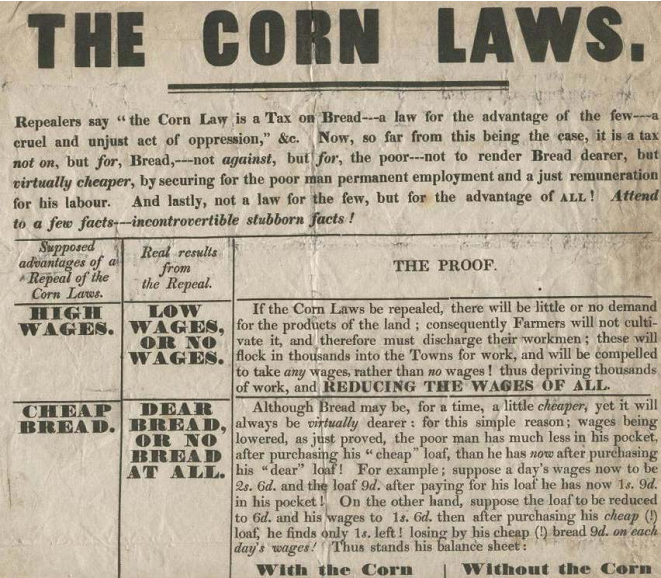
\includegraphics[scale=0.5]{fig/sfm/lec4-1}
\end{column}
\end{columns}

\end{frame}

\begin{frame}{Historical Example: Corn Laws }

\begin{itemize}
\item Efforts to overturn the Importation Act were championed by industrialists
and entrepreneurs 

\begin{itemize}
\item Anti -Corn Law League 
\item James Wilson 
\end{itemize}
\item In their view, higher corn prices increased wages paid to industrial
workers and decreased their profits 
\item And tariff retaliation from abroad hurt them too (since Britain exported
manufactures) 
\item Corn Laws were finally repealed in 1846 due to a large extent to the
Irish Potato Famine
\end{itemize}
\end{frame}

\begin{frame}{Derived Questions }



\begin{itemize}
\item Why were landowners so eager to maintain import protection for corn? 
\item Why were industrialists so opposed to it? 
\item Was the effect of the Corn Laws negative for workers (as some claim)
or was it actually positive? 
\item What was the effect of the Corn Laws for aggregate welfare in Britain? 
\item Why did it take so long to repeal the Corn Laws? 
\end{itemize}
\end{frame}

\begin{frame}{Specific Factor Model的Mission}
	\begin{itemize}
		\item 对于以上问题,SFM有着极强的解释力
		\item So far,我们已经通过Ricardian Model理解了“Trade is Great"
		\item The remainning questions:(1)谁会从贸易中获益;(2)谁会从贸易中受损;(3)在什么情况下收益或受损?
	\end{itemize}

\end{frame}

\section{A Formal Model}
\begin{frame}{Intellectual History }

\begin{itemize}
\item Specific Factors Model is sometimes referred to as the Ricardo- Viner 
\item Was independently formalized by Ronald W. Jones (1931 - ) and Paul
Samuelson (1915 -2009) in 1971
\begin{figure}


\centering{}
\includegraphics[width=3cm]{fig/sfm/lec4-2}%
\begin{minipage}[t]{1\columnwidth}%
%
\end{minipage} 
\includegraphics[width=3cm]{fig/sfm/lec4-3}
\end{figure}

\end{itemize}
\end{frame}



\section{Setup of the Model}
\begin{frame}{Assumptions of the Model }

\begin{itemize}
\item Two - country world with a Home country and a Foreign one 
\item Only two goods are relevant for production and consumption (cloth
and food) 
\item Three factors of production: labor ($L$ ), capital ($K$) and land
( $T$ for terrain) all in fixed supply 
\item Cloth is produced with labor and capital, but not land 
\item Food is produced with labor and land, but not capital 
\item Labor can move freely across sectors
\item All markets are perfectly competitive 
\end{itemize}
\end{frame}

\begin{frame}{Technology}

\begin{itemize}
\item The production function for cloth gives the quantity of cloth that
can be produced given any input of capital and labor: 
\[
Q_{C}=Q_{C}(K,L_{C})
\]


\begin{itemize}
\item $Q_{C}$ is the output of cloth 
\item $K$ is the capital stock 
\item $L_{C}$ is the labor force employed in cloth 
\end{itemize}
\item We will assume that it features constant returns to scale and diminishing
marginal products 
\end{itemize}
\end{frame}

\begin{frame}{Technology (cont.) }

\begin{itemize}
\item Similarly, the production function for food gives the quantity of
food that can be produced given any input of land and labor:
\[
Q_{F}=Q_{F}(T,L_{F})
\]
 
\item $Q_{F}$ is the output of food
\item $T$ is the supply of land 
\item $L_{F}$ is the labor force employed in food 
\item And again, it features constant returns to scale and diminishing marginal
products
\end{itemize}
\end{frame}

\begin{frame}{Constant Returns to Scale}

\begin{itemize}
\item If one increases all factors by the same proportion, output increases
by the same proportion, or 
\[
Q_{C}(aK,aL_{C})=aQ_{C}(K,L_{C})
\]
 
\item Mathematically, $Q_{C}$ is homogenous of degree one in $K$ and $L_{C}$ 
\item Note that the technology in the Ricardian model also featured constant
returns to scale, though in that case there was only one factor of
production 
\end{itemize}
\end{frame}

\begin{frame}{Diminishing Marginal Product of Labor }


\begin{columns}[onlytextwidth]
\begin{column}{0.4\textwidth}
\begin{itemize}
\item The larger is the amount of labor used in cloth, the lower the increase
in output from an increase in labor
\item So the marginal product of labor is decreasing in $L_{C}$ or $\partial(\partial F_{C}/\partial L_{C})/\partial L_{C}<0$
\end{itemize}

\end{column}
\begin{column}{0.6\textwidth}
\centering 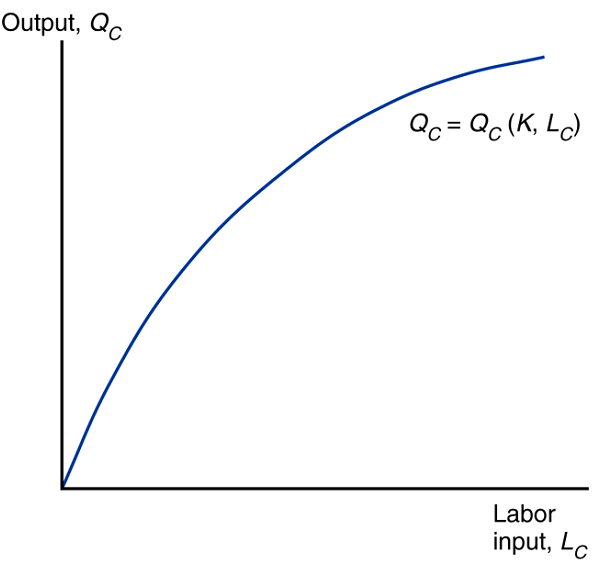
\includegraphics[width=0.7\columnwidth]{fig/sfm/lec4-5}
\end{column}
\end{columns}

\end{frame}

\begin{frame}{Diminishing Marginal Product of Labor}


\begin{columns}[onlytextwidth]
\begin{column}{0.4\textwidth}
\begin{itemize}
\item Why are returns diminishing? 
\item When $L_{C}$ increases (for a given $K$), each worker has less and
less capital to work with 
\item The same is true with labor and land in food production
\end{itemize}

\end{column}
\begin{column}{0.6\textwidth}
\centering 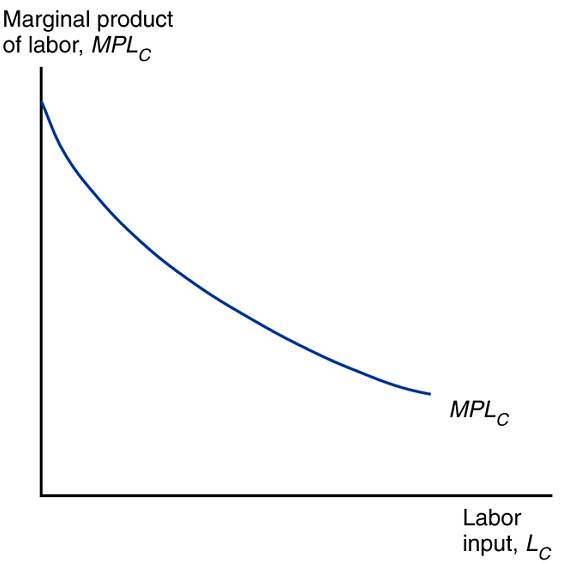
\includegraphics[width=0.7\columnwidth]{fig/sfm/lec4-6}
\end{column}
\end{columns}


\end{frame}

\begin{frame}{Discussion of Assumptions}

\begin{itemize}
\item The model captures that, in the short - run, some factors are more
flexible than others 

\begin{itemize}
\item They can move from employment in one sector to another more quickly
or at a lower cost 
\end{itemize}
\item Example of labor and capital: 

\begin{itemize}
\item In the U.S., a displaced worker (relative to a non -displaced one)
has a lower probability of being employed for the next 4 years following
displacement 
\item In comparison, capital depreciates over 15 -20 years and structures
over 30-50 years 
\end{itemize}
\end{itemize}
\end{frame}

\begin{frame}{Discussion of Assumptions (cont.)}

\begin{itemize}
\item In the short/medium- run, labor thus appears to be more flexible than
capital across sectors 
\item The Specific Factors model captures the effects of trade in this short/medium-
run time frame (5- 15 years) where capital is fixed in each sector
but labor is flexible (can move between sectors) 
\item Specific factors in the model will be capital and land, but you might
find it more useful to think of these as representing different types
of physical or human capital 
\end{itemize}
\end{frame}

\begin{frame}{Production Possibility Frontier}

\begin{itemize}
\item Formally, we want to characterize the combinations of $Q_{C}=Q_{C}(K,L_{C})$
and $Q_{F}=Q_{F}(T,L_{F})$ that satisfy 
\[
L_{C}+L_{F}=L
\]

\item It is clear that $(0,Q_{F}(T,L))$ and$(Q_{C}(K,L),0)$ are two points
in the PPF 
\item What shape does the PPF take? Is it linear as in the Ricardian model? 
\end{itemize}
\end{frame}

\begin{frame}{Shape of the PPF: Heuristic Derivation}


\begin{columns}[onlytextwidth]
\begin{column}{0.4\textwidth}
\begin{itemize}
\item Suppose PPF was linear  Then the point M given by $(\frac12 Q_{C}(K,L),\frac12 Q_{F}(T,L))$
would be on the PPF too 
\item But note that (why?) 
\[
Q_{C}(K,\text{½}L)>\text{½}Q_{C}(K,L)
\]
\[
Q_{F}(T,\text{½}L)>\text{½}Q_{F}(T,L)
\]

\item So we can produce strictly more by allocating $\frac12$ of labor
to each sector 
\end{itemize}

\end{column}
\begin{column}{0.6\textwidth}
\centering  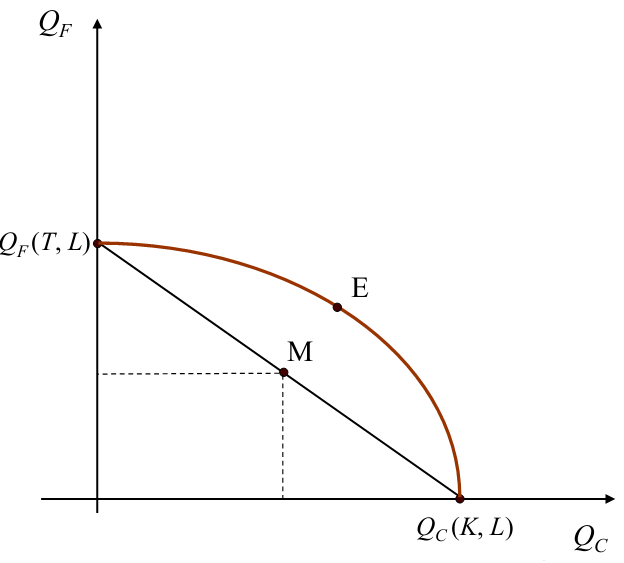
\includegraphics[width=0.6\columnwidth]{fig/sfm/lec4-7}
\end{column}
\end{columns}

\end{frame}

\begin{frame}{Graphical Derivation}


\begin{figure}


\centering{}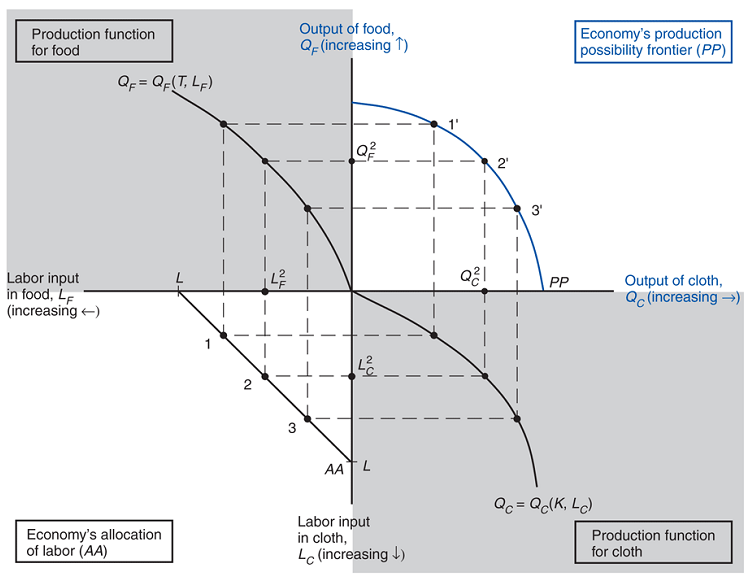
\includegraphics[width=7cm]{fig/sfm/lec4-8}
\end{figure}

\end{frame}

\begin{frame}{Opportunity Costs and the PPF }

\begin{itemize}
\item Notice an important difference from the Ricardian model 
\item The opportunity cost of producing cloth in terms of food is not constant
in this model: 

\begin{itemize}
\item it is \textbf{\textcolor{blue}{low}} when the economy produces very
little cloth and a lot of food 
\item But it is \textbf{\textcolor{blue}{high}} when the economy produces
a lot of cloth and little food 
\end{itemize}
\item Opportunity cost of producing a unit of cloth is $MPL_{F}/MPL_{C}$
units of food (since only labor input is moving along the PPF)
\item Remember that the slope of the PPF measures this opportunity cost
(we’ll come back to this) 
\end{itemize}
\end{frame}

\begin{frame}{Sketch of Supply Side Equilibrium }


\begin{columns}[onlytextwidth]
\begin{column}{0.5\textwidth}
\begin{itemize}
\item Perfect competition and profit maximization will imply that the economy
will produce at the point that maximizes the value of production,
$V$: 
\[
V=P_{C}Q_{C}+P_{F}Q_{F}
\]
 
\item $P_{C}$ is the price of cloth and $P_{F}$ is the price of food 
\item But this implies that the production point will be such that the slope
of the PPF ($-dQ_{F}/dQ_{C}$ ) equals the relative price ratio $P_{C}/P_{F}$ 
\end{itemize}

\end{column}
\begin{column}{0.5\textwidth}
\centering 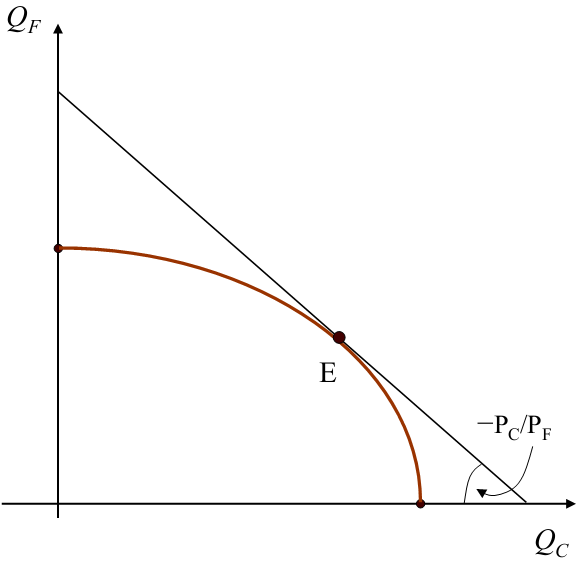
\includegraphics[width=0.7\columnwidth]{fig/sfm/lec4-9}
\end{column}
\end{columns}

\end{frame}

\begin{frame}{Sketch of General Equilibrium}


\begin{columns}[onlytextwidth]
\begin{column}{0.5\textwidth}
\begin{itemize}
\item Suppose that preferences are such that they can be represented by
those of a representative consumer
\item Then optimality on the demand side requires the marginal rate of substitution
(i.e, the slope of the “social” indifference curve) to equal the relative
price $P_{C}/P_{F}$ 
\item So both supply-side factors and demand -side factors affect relative
prices 
\item We will focus on supply-side differences across countries 
\end{itemize}

\end{column}
\begin{column}{0.5\textwidth}
\centering 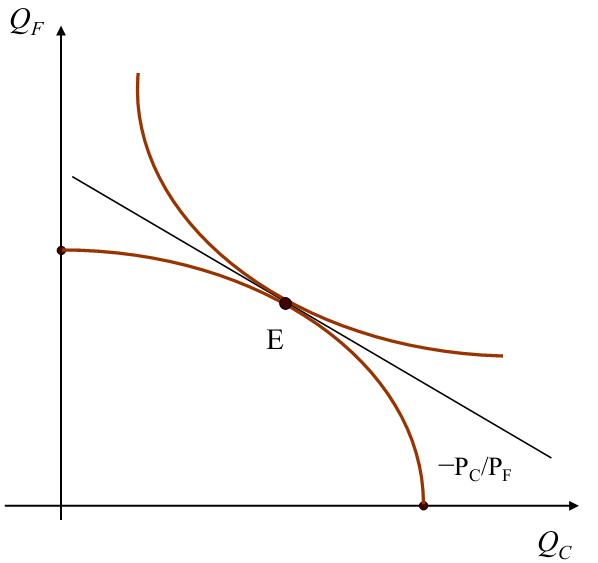
\includegraphics[width=0.7\columnwidth]{fig/sfm/lec4-10}
\end{column}
\end{columns}

\end{frame}

\begin{frame}{Map the Equilibrium }

\begin{itemize}
\item Having described the PPF, we will next discuss how the general equilibrium
is actually determined 
\item First, we will study the allocation of labor across sectors 
\item Then we will trace its implications for the relative supply schedule 
\item And finally we will determine relative prices as the intersection
of the relative supply and relative demand schedules (as in the Ricardian
model) 
\end{itemize}
\end{frame}



\section{Allocation of labor across sectors劳动力如何在两个部门进行配置}
\begin{frame}{Allocation of Labor }

\begin{itemize}
\item How much labor is employed in each sector? 

\begin{itemize}
\item Results from equilibrium between supply and demand in the labor market 
\end{itemize}
\item Demand for labor: 

\begin{itemize}
\item In each sector, employers will maximize profits by demanding labor
up to the point where the value produced by an additional hour equals
the marginal cost of employing a worker for that hour 
\item Demand curve for labor in the cloth sector: $MPL_{C}\times P_{C}=w$ 
\item Demand curve for labor in the food sector: $MPL_{F}\times P_{F}=w$ 
\end{itemize}
\end{itemize}
\end{frame}

\begin{frame}{Remember Diminishing MPL}


\begin{figure}


\begin{centering}
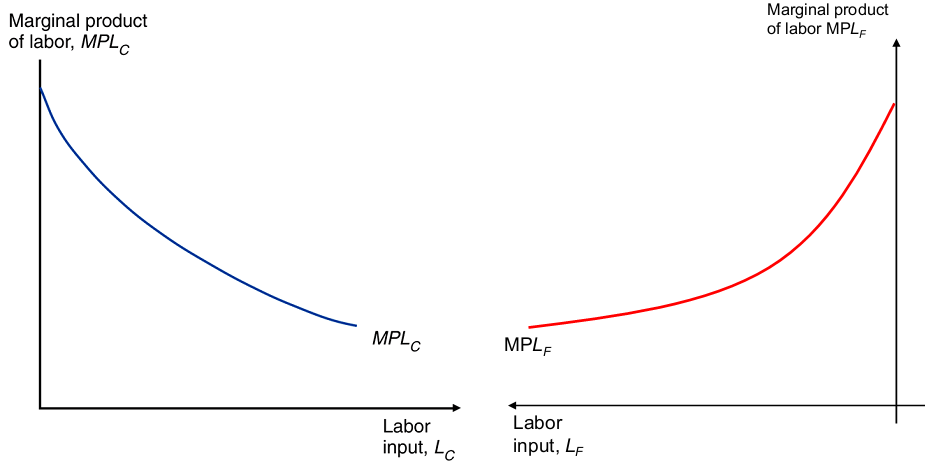
\includegraphics[width=12cm]{fig/sfm/lec4-11}
\par\end{centering}

\end{figure}

\end{frame}

\begin{frame}{Combining Them! }


\begin{figure}


\begin{centering}
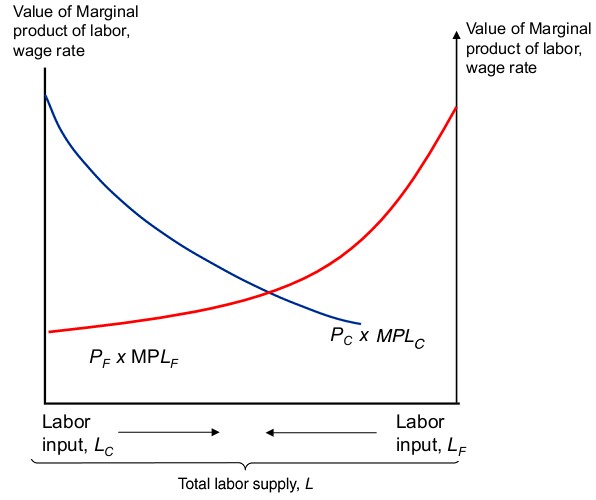
\includegraphics[width=8cm]{fig/sfm/lec4-12}
\par\end{centering}

\end{figure}

\end{frame}

\begin{frame}{Equilibrium in Labor Market }


\begin{columns}[onlytextwidth]
\begin{column}{0.3\textwidth}
\begin{itemize}
\item The two sectors must pay the same wage because labor can move between
sectors 
\item Where the labor demand curves intersect gives the equilibrium wage
and allocation of labor between the two sectors 
\end{itemize}

\end{column}
\begin{column}{0.7\textwidth}
\centering 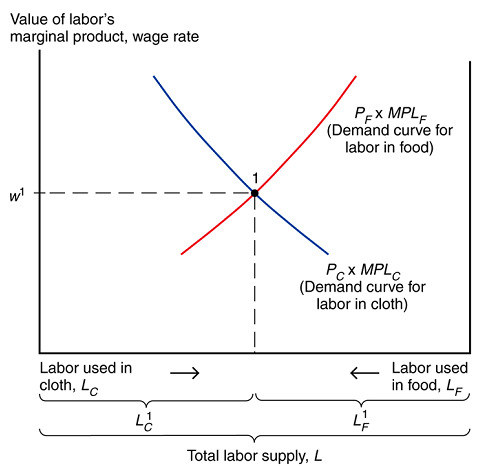
\includegraphics[width=0.6\columnwidth]{fig/sfm/lec4-13}
\end{column}
\end{columns}

\end{frame}

\begin{frame}{Equilibrium }


\begin{columns}[onlytextwidth]
\begin{column}{0.4\textwidth}
\begin{itemize}
\item Notice that in equilibrium 
\[
-MPL_{F}/MPL_{C}=-P_{C}/P_{F}
\]

\item So the allocation of labor is such that the production possibility
frontier must be tangent to a line whose slope is minus the price
of cloth divided by that of food, as anticipated earlier 
\end{itemize}

\end{column}
\begin{column}{0.6\textwidth}
\centering 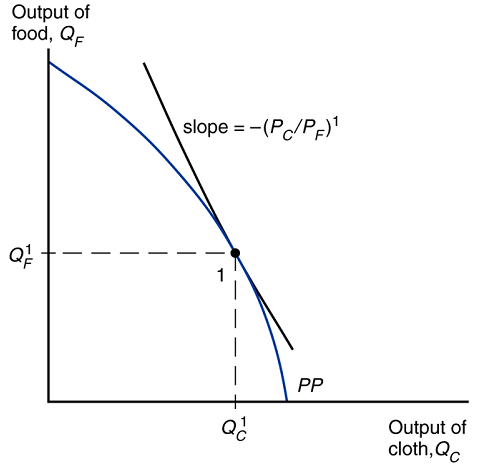
\includegraphics[width=0.7\columnwidth]{fig/sfm/lec4-14}
\end{column}
\end{columns}

\end{frame}




\begin{frame}{Deriving the Relative Supply Schedule}


\begin{columns}[onlytextwidth]
\begin{column}{0.4\textwidth}
\begin{itemize}
\item Suppose that $P_{C}/P_{F}$ rises 
\item This will increase the production of cloth and decrease the production
of food (more on this later) 
\item The effect is smooth
\end{itemize}

\end{column}
\begin{column}{0.6\textwidth}
\centering 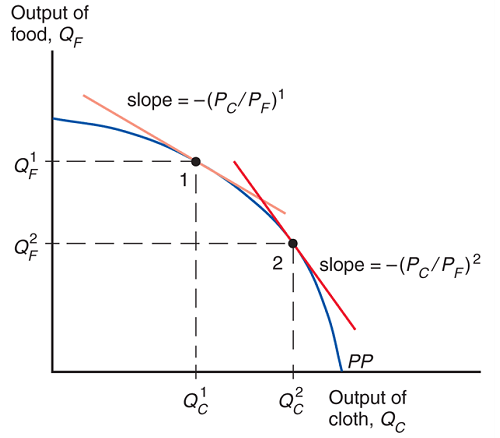
\includegraphics[width=0.7\columnwidth]{fig/sfm/lec4-15}
\end{column}
\end{columns}

\end{frame}

\begin{frame}{General Equilibrium }


\begin{figure}


\centering{}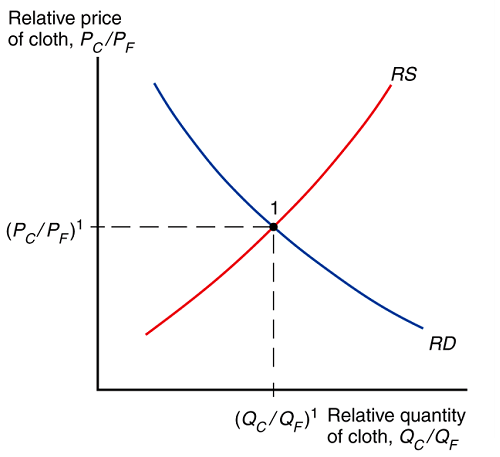
\includegraphics[width=8cm]{fig/sfm/lec4-16}
\end{figure}

\end{frame}



\section{比较静态分析}
\subsection{Comparative Statics I: Price Change}
\begin{frame}{Prices, Wages and Labor Allocation}

\begin{itemize}
\item What happens to the allocation of labor and the distribution of income
when the prices of food and cloth change? 
\item Two cases: 

\begin{enumerate}
\item An equal proportional change in prices 
\item A change in relative prices 
\end{enumerate}
\end{itemize}
\end{frame}

\begin{frame}{A Proportional Change in Prices}


\begin{columns}[onlytextwidth]
\begin{column}{0.4\textwidth}
\begin{itemize}
\item No real changes occur 
\item The wage rate ($w$) rises in the same proportion as the prices, so
\textbf{\textcolor{blue}{real wages}} are unaffected 
\item The real incomes of capital owners and landowners also remain the
same 
\end{itemize}

\end{column}
\begin{column}{0.6\textwidth}
\centering 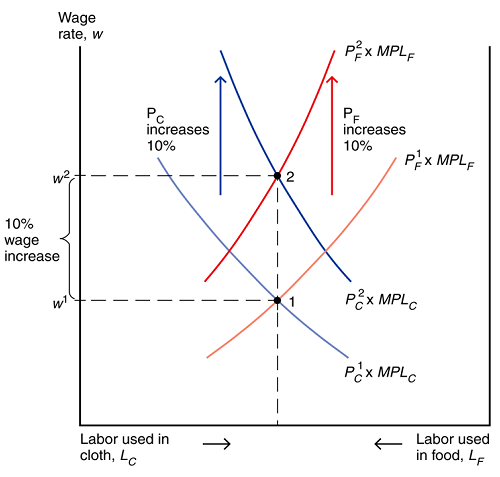
\includegraphics[width=0.7\columnwidth]{fig/sfm/lec4-17}
\end{column}
\end{columns}

\end{frame}

\begin{frame}{An Increase in Relative Price of Cloth }


\begin{columns}[onlytextwidth]
\begin{column}{0.4\textwidth}
\begin{itemize}
\item When only $P_{C}$ rises, labor shifts from the food sector to the
cloth sector and output of cloth rises while that of food falls 
\item Relative supply of cloth and food is thus (smoothly) increasing in
the relative price $P_{C}/P_{F}$
\end{itemize}

\end{column}
\begin{column}{0.6\textwidth}
\centering 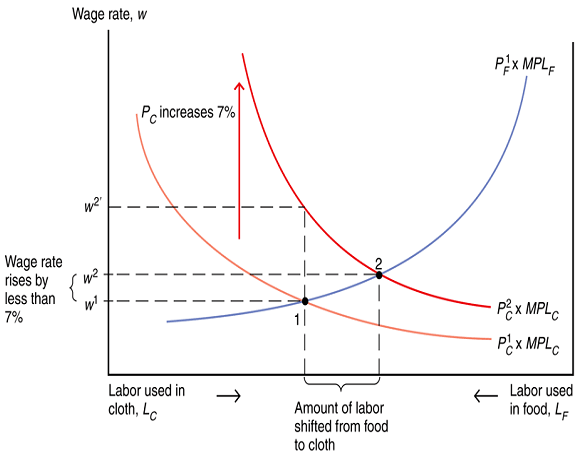
\includegraphics[width=0.9\columnwidth]{fig/sfm/lec4-18}
\end{column}
\end{columns}

\end{frame}

\begin{frame}{Effect on Income Distribution }

\begin{itemize}
\item Note that the wage rate ($w$) does not rise as much as $P_{C}$ because
cloth employment increases and thus the marginal product of labor
in that sector falls ($MPL_{C}$ falls) 
\item On the other hand, the wage rate ($w$ ) rises relative to the price
of food $P_{F}$ (since $MPL_{F}$ rises) 
\item The effect on the purchasing power of wages (or real wages) is thus
\textbf{\textcolor{blue}{ambiguous}} and depends on the relative importance
of cloth and food in workers’ consumption
\end{itemize}
\end{frame}

\begin{frame}{Effect on Income Distribution}

\begin{itemize}
\item Owners of capital are definitely better off 
\item $P_{C}/w$ rises and so does their volume of production 
\item Landowners are definitely worse off 
\item $P_{F}/w$ falls and so does their volume of production 
\item \textbf{\textcolor{blue}{General principle}}: changes in relative
prices lead to distributional conflict between the owners of different
specific factors 
\end{itemize}
\end{frame}



\subsection{Comparative Statics II: Factor Change}
\begin{frame}{Changes in the Specific Factors}


\begin{columns}[onlytextwidth]
\begin{column}{0.4\textwidth}
\begin{itemize}
\item Suppose the endowment of capital increases 
\item Labor moves from food production to cloth production 
\item Relative output of cloth goes up and relative price $P_{C}/P_{F}$
goes down 
\end{itemize}

\end{column}
\begin{column}{0.6\textwidth}
\centering 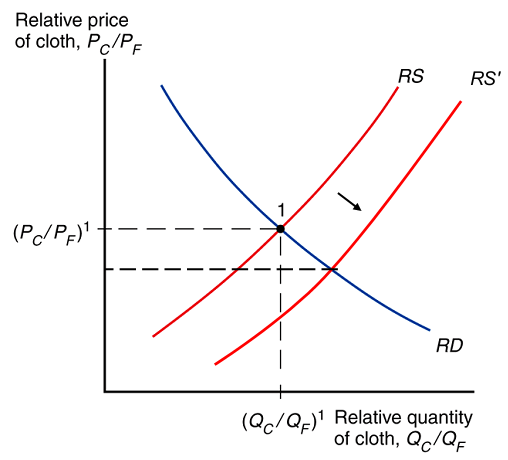
\includegraphics[width=0.8\columnwidth]{fig/sfm/lec4-19}
\end{column}
\end{columns}

\end{frame}

\begin{frame}{Changes in the Specific Factors}


\begin{columns}[onlytextwidth]
\begin{column}{0.4\textwidth}
\begin{itemize}
\item Suppose the endowment of land increases 
\item Labor moves from cloth production to food production 
\item Relative output of cloth goes down and relative price $P_{C}/P_{F}$
goes up
\end{itemize}

\end{column}
\begin{column}{0.6\textwidth}
\centering 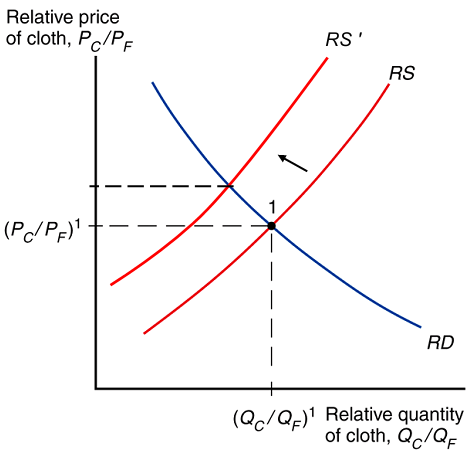
\includegraphics[width=0.8\columnwidth]{fig/sfm/lec4-20}
\end{column}
\end{columns}

\end{frame}

\section{特定要素模型中的国际贸易}
\begin{frame}{International Trade }

\begin{itemize}
\item Suppose Home has more capital but less land than Foreign 
\item For simplicity assume that both countries have the same labor force
In which country will the relative price of cloth $P_{C}/P_{F}$ under
autarky be higher? 
\item Which country has comparative advantage in the production of cloth?
\end{itemize}
\end{frame}

\begin{frame}{International Trade}


\begin{columns}[onlytextwidth]
\begin{column}{0.4\textwidth}
\begin{itemize}
\item From the point of view of Home, trade opening is analogous to an increase
in the relative price $P_{C}/P_{F}$
\item This is because the world relative price will need to settle somewhere
between the two autarky relative prices 
\end{itemize}

\end{column}
\begin{column}{0.6\textwidth}
\centering 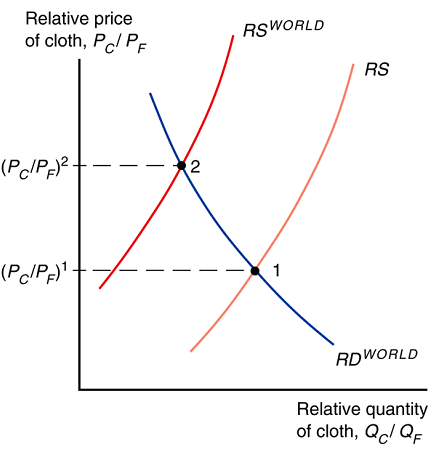
\includegraphics[width=0.7\columnwidth]{fig/sfm/lec4-21}
\end{column}
\end{columns}

\end{frame}

\begin{frame}{Pattern of Trade}

\begin{itemize}
\item Because $(P_{C}/P_{F})^{W}>P_{C}/P_{F}$ , with trade, \textbf{\textcolor{blue}{Home’s}}
relative supply of cloth is higher than its relative demand 

\begin{itemize}
\item Hence, it will export cloth and import food 
\end{itemize}
\item Conversely, because $(P_{C}/P_{F})^{*}>(P_{C}/P_{F})^{W}$ ,\textbf{\textcolor{blue}{{}
Foreign’s}} relative supply of cloth is lower than its relative demand 

\begin{itemize}
\item Hence, it will export food and import cloth 
\end{itemize}
\item \textbf{\textcolor{blue}{In general}}, the pattern of trade depends
in a complicated manner on the endowments of all factors 

\begin{itemize}
\item but holding constant L and one of the specific factors, the good in
the other sector will be exported by the country with the largest
endowment of the factor specific to that sector 
\end{itemize}
\end{itemize}
\end{frame}

\begin{frame}{Gains from Trade }


\begin{columns}[onlytextwidth]
\begin{column}{0.4\textwidth}
\begin{itemize}
\item The economy as a whole gains from trade 
\item Trade allows the mix of cloth and food consumed to differ from the
mix produced 
\item Home is able to afford amounts of cloth and food that the country
is not able to produce itself 
\end{itemize}

\end{column}
\begin{column}{0.6\textwidth}
\centering 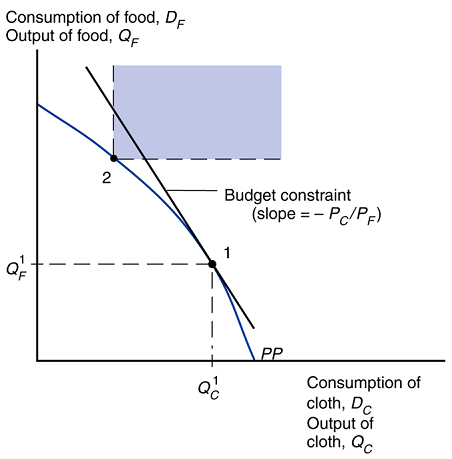
\includegraphics[width=0.6\columnwidth]{fig/sfm/lec4-22}
\end{column}
\end{columns}

\end{frame}

\begin{frame}{Trade and Income Distribution}

\begin{itemize}
\item From our previous discussion, trade opening: 

\begin{itemize}
\item benefits Home capitalists 
\item hurts Home landowners
\item has an ambiguous effect on Home workers 
\end{itemize}
\item \textbf{\textcolor{blue}{General principle: }}trade benefits the factor
that is specific to the export sector of each country, but hurts the
factor that is specific to the import-competing sectors 
\item But with appropriate redistribution, everybody could be made better
off
\end{itemize}
\end{frame}

\begin{frame}{Terms of Trade Effects}

\begin{itemize}
\item The ratio of the price of the exported good to the price ofthe imported
good is referred to as a country's \textbf{\textcolor{blue}{terms
of trade}}

\begin{itemize}
\item For the home, it is $P_{C}/P_{F}$. Conversely for the foreign.
\end{itemize}
\item As in the Ricardian model, improvements in the terms of trade (due
for instance to proportional or import - biased growth in Foreign)
will enhance aggregate welfare 
\item But now they will also lead to distributional conflict 
\item Owners of the specific factor in the import- sector will be hurt by
improvements in the terms of trade 
\end{itemize}
\end{frame}

\begin{frame}{Domestic Growth}


\begin{columns}[onlytextwidth]
\begin{column}{0.4\textwidth}
\begin{itemize}
\item Holding constant the terms of trade, domestic increases in the endowments
of specific factors will hurt both specific factors but will benefit
labor
\end{itemize}

\end{column}
\begin{column}{0.6\textwidth}
\centering 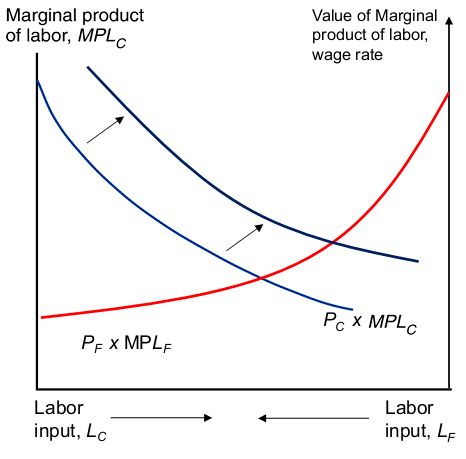
\includegraphics[width=0.8\columnwidth]{fig/sfm/lec4-23}
\end{column}
\end{columns}


\end{frame}



\subsection{Effects of Tariff and rethinking Corn Laws}
\begin{frame}{Effects of Tariff Protection}

\begin{itemize}
\item We have argued that a move to free trade will move relative prices
from their autarky level to the level in world markets 
\item If a country sets a tariff on its imports, then this will be analogous
to a move of its relative prices back to a level closer to its autarky
level 
\item Two caveats: 

\begin{itemize}
\item This will also generate tariff revenue, so effects are more involved 
\item If a country is large enough, its tariffs might affect world prices 
\item We will come back to these issues later in the course 
\end{itemize}
\end{itemize}
\end{frame}

\begin{frame}{Back to Corn Laws }

\begin{itemize}
\item Because Britain was a net exporter of manufactures and a net importer
of cereal products, it is not surprising that: 

\begin{itemize}
\item Landowners favored import protection of cereal products 
\item Capitalists or industrialists opposed it 
\item Workers had ambivalent views
\end{itemize}
\item Yet, it seems that industrial workers tended to oppose it, while land
laborers tended to favored it 

\begin{itemize}
\item Why?
\end{itemize}
\end{itemize}
\end{frame}

\begin{frame}{The Short -Run }

\begin{itemize}
\item Suppose that workers could not relocate across sectors immediately
after trade opening 
\item What would be the impact of trade on their welfare? 
\item Depends on the sector in which the worker is employed 
\item Then welfare of \textbf{\textcolor{blue}{both factors}} in the comparative
advantage sector rises, and the welfare of \textbf{\textcolor{blue}{both
factors}} in the other sector falls 

\begin{itemize}
\item Same as in an endowment economy where each factor’s endowment is entirely
composed of the good in the sector where that factor is 
\end{itemize}
\end{itemize}
\end{frame}

\begin{frame}{The Long -Run }

\begin{itemize}
\item Think of land now as a type of physical capital that is specific to
food production, but that with time can be converted into the type
of physical capital used in the production of cloth 
\item The equilibrium in the long - run is thus analogous to that in a two
- factor model in which both factors are freely mobile across sectors 

\begin{itemize}
\item Do we then go back to the predictions of the Ricardian model? 
\item Do distributional effects of trade vanish? 
\end{itemize}
\end{itemize}
\end{frame}






\begin{frame}{Agenda for Next Week}

\begin{itemize}
 \item Trade and Resources: The Heckscher-Ohlin Model
	
	\begin{itemize}
		\item Heckscher-Ohlin Model (I). Motivation. Model Assumptions and Autarky
		Equilibrium
		\item Heckscher-Ohlin Model (II). Trade Equilibrium, Comparative Statics
		and Empirical Evidence
		\item Heckscher-Ohlin Model (III). An Application: The Trade and Wages Debate. 
	\end{itemize}
 \item Readings: 
	
	\begin{itemize}
		\item K-O-M Chapter 4 and 5 
		\item F-T Chapter 4
	\end{itemize}
\end{itemize}
\end{frame}

\end{document}
